\section{Bag of Words (BoW)}
BoW (Bag of Words), metindeki kelimelerin frekansına bakarak metinler arasında benzerlik ölçer. Kelime sırasını ve gramer yapılarını dikkate almaz sadece frekansa bakar. Metinlerin uzunluğuna bağlı değildir. BoW, bir metindeki her kelimenin varlığını veya sıklığını temsil eden bir vektör oluşturur. Her kelime, metinde kaç kez geçtiğine veya metinde geçip geçmediğine bağlı olarak bir özellik olarak temsil edilir. Veri setindeki geçen tüm farklı kelimeler için bir sözlük oluşturulur. Her bir metin için, sözlükte her kelimenin sıklığına göre bir vektör oluşturulur.  

\begin{figure}[h]
    \centering
    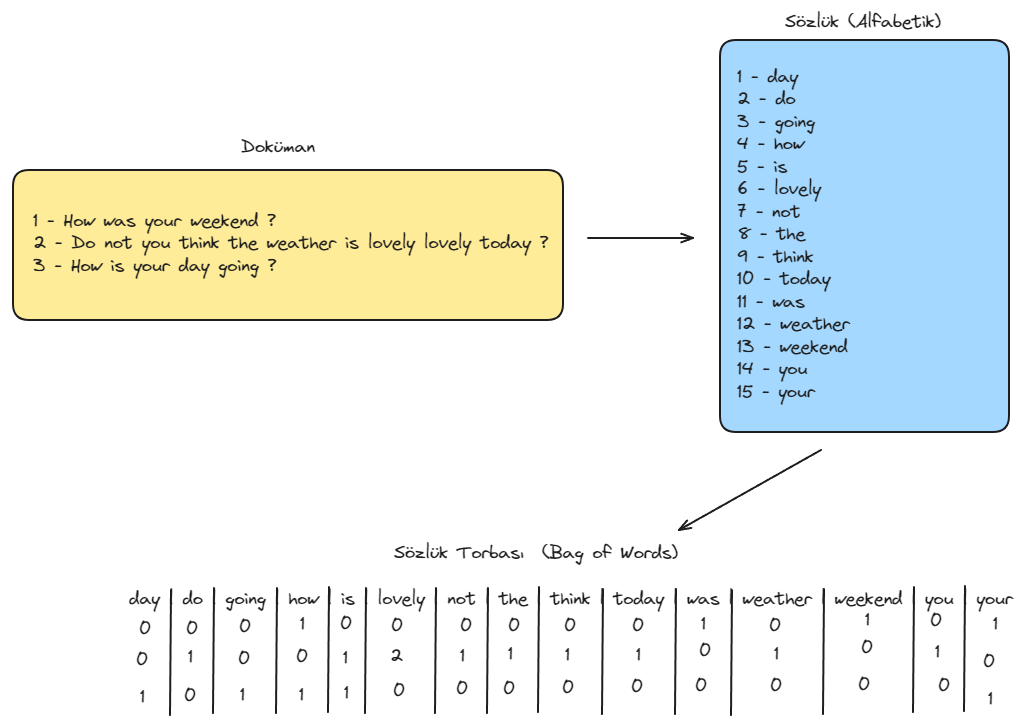
\includegraphics[width=1\textwidth]{images/bag_of_words.png}
    \caption{Sözlük torbası.}
    \label{fig:enter-label}
\end{figure}

\subsection{Python Kodu}

\begin{lstlisting}[language=Python]
from sklearn.feature_extraction.text import CountVectorizer

# Ornek metin veri seti
corpus = [
    # [0 0 0 1 0 0 0 0 0 0 1 0 1 0 1]
    "How was your weekend ?",
    # [0 1 0 0 1 2 1 1 1 1 0 1 0 1 0]
    "Do not you think the weather is lovely lovely today ?",
    # [1 0 1 1 1 0 0 0 0 0 0 0 0 0 1]
    "How is your day going ?"
]

# CountVectorizer kullanarak BoW vektorlerini olusturma
vectorizer = CountVectorizer()
X = vectorizer.fit_transform(corpus)

# Olusturulan BoW matrisini ekrana yazdirma
print("BoW Matrisi:")
print(X.toarray())

# Sozluk (kelimeler) listesini ekrana yazdirma
# ['day', 'do', 'going', 'how', 'is', 'lovely', 'not', 'the', 'think', 'today', 'was', 'weather', 'weekend', 'you', 'your']
print("Sozluk (Kelimeler):")
print(vectorizer.get_feature_names_out())
\end{lstlisting}

\newpage